

%-------------------------

\newpage


\section{Fieldwork elements}{Elements de terrain}

\label{sec:qualitative}


%-------------------------


Cette section propose d'illustrer la problématique des interactions entre réseaux de transports et territoires, et plus particulièrement leur complexité\comment[FL]{au fait je n'y pense que la : tu n'as pas defini reellement ``reseaux de transport''} et la diversité des situations possibles déjà perceptibles de manière subjective à l'échelle microscopique, par des exemples concrets de terrain.\comment[FL]{quali $\neq$ subjectif L'idée dans une these est qu'il n'y ait rien de subjectif (a part si c'est explicitement dit)} Le terrain géographique majoritaire\comment[FL]{formulation ambigue : il y aura autre chose ? pourquoi ?} est le Delta de la Rivière des Perles en Chine (\cn{珠江三角洲}), dans la province du Guangdong (\cn{广东}), que nous avons décrit ci-dessus, et plus particulièrement en grande partie la ville de Zhuhai (\cn{珠海}). Des observations ont également été effectuées en métropole Parisienne. Nous assumons le terme de \emph{Terrain géographique}, en toute conscience des débats épistémologiques que peuvent poser l'utilisation de celui-ci. En effet,

Dans le cadre du projet européen Medium\footnote{Le project Medium, qui met en partenariat des université européennes et chinoise, s'intitule ``\textit{New pathways for sustainable urban development in China’s medium-sized cities}. Il vise à étudier la soutenabilité selon un prisme interdisciplinaire et multidimensionnel, dans le cas de zones urbaines en forte croissance. Trois villes moyennes chinoise ont été choisies comme cas d'étude. Voir \url{http://mediumcities-china.org/} pour plus d'information.}, visant à une approche interdisciplinaire de la soutenabilité pour les villes Chinoises en se concentrant sur les villes moyennes, cette ville a été choisie comme cas d'étude\comment[FL]{ce n'est pas pertinent ici}. Lorsque la source n'est pas explicitement précisée, les observations proviennent du travail de terrain, pour lequel des compte-rendus narratifs sont disponibles en Annexe~\ref{app:sec:qualitative}. Le format de ceux-ci est ``à-la-volée'' suivant les recommandations de \cite{goffman1989fieldwork} pour la prise de notes en terrain d'immersion notamment, tandis que la position volontairement subjective rejoint \cite{ball1990self} qui souligne l'importance de la réflexivité pour tirer des conclusions rigoureuses à partir d'observations qualitatives de terrain duquel le chercheur est partie intégrante.\comment[FL]{oui si cela concerne un milieu social petit. mais pour ce qui concerne des visites de terrains dns des grandes villes, je ne vois pas la boucle de retroaction observateur $\implies$ systeme}




%----------------------------



%%%%%%%%%%%%%%%%%%%%%
\subsection{Transportation network development}{Développement d'un réseau de transport}



\bpar{
One main axis of the fieldwork research in China was to get a subjective view of multiple aspects and layers of the complex and ever-changing public transportation system, in Zhuhai as an illustration for local transportation but also at larger scales in China. Indeed, transportation network modeling or data analysis such as accessibility studies or land-use transport interaction models I develop as the main focus of my thesis, generally fail to grasp microscopic aspects that can become crucial when it comes to the effective use of the network. For example, multimodality can be made effective in practice through self-organized informal transportation modes that solve the ``last-mile'' kilometer problem~\cite{liu2012solving} that seems to be often forgotten in the planning of newly developed areas in China. Or in the contrary, practical details such as ticket booking or check-in delays can drastically change use patterns.
}{
L'un des axes principaux de la recherche de terrain en Chine\comment[FL]{tu ne dis pas ce que tu cherches. on ne fait pas de terrain sans raison !} a été de construire une vue subjective des multiples facettes et couches d'un système de transport public complexe et en mutation permanente. La portée des observations s'étend sur Zhuhai comme illustration des transports locaux mais aussi ponctuellement sur d'autres régions en Chine. Ces observations ont une logique propre en comparaison de la modélisation des réseaux de transport ou l'analyse de données, comme des études d'accessibilité ou des modèles d'interaction entre usage du sol et transport, qui seront menés par la suite. En effet, celles-ci échouent généralement a capturer des aspects microscopiques\comment[FL]{def} qui peuvent devenir cruciaux au regard de l'utilisation effective du réseau. Par exemple, la multi-modalité\comment[FL]{def} peut être rendue efficace en pratique par l'emergence de modes de transports auto-organisés informels, ou la mise en place de nouveaux modes comme le vélo en partage, ce qui résout le ``problème du dernier kilomètre''~\cite{liu2012solving}, qui semble être souvent négligé dans la planification de zones nouvellement développées en Chine. Au contraire, des details pratiques comme la réservation des tickets ou les délais d'enregistrement à l'embarquement peuvent influencer considérablement les motifs d'usage.
}


\bpar{
I made several trips to understand how the High-speed rail (HSR) network works. Since 2008, China has achieved the largest HSR network starting from nothing, with a huge success and currently saturated lines. These answer to primary demand patterns in terms of city size, but other dimensions have been taken into account in their planning, such as the development of tourism. This way, the Guangzhou-Shenyang line has seen the construction of stations specific to the development of tourism, such as Yangshuo in Guanxi province that has seen its frequentation strongly rising. One year after the station opened, the road link with the city is still in construction, but most of trains stop in the week-end – more than one per hour, and are full more than two weeks in advance. New patterns of mobility must be induced by this new offer, as shown by a Guangzhou inhabitant I interviewed in Yangshuo, that was coming with co-workers just for the week-end as a ``team-building'' trip financed by their startup in information technology. I observed a similar strategy must have been employed for the line Chengdu-Emeishan, which principal objective for now is to desserve the highly visited touristic destination of Leshan and Emeishan, although the missing link from Leshan to Guiyang is already well advanced and will complete the direct link between Guangzhou and Changdu \cite{lu2012chengdu}. The complexity of the network is increased by the diversity of missions and congestion, and maximal potential speeds seem to be not systematically exploited.
}{
Différents voyages sur le territoire Chinois ont été effectués pour percevoir les mécanismes d'usage\comment[FL]{quel sens donnes-tu à cela ?} du réseau à grande vitesse.\comment[AB]{tu décris le protocole de selection des parcours en annexe ?} Depuis 2008, la Chine a établi le plus grand réseau de HSR du monde à partir de zéro, qui a connu un grand succès et dont les lignes sont actuellement saturées.\comment[FL]{quel apport / problematique} Celui-ci répond à des motifs de demande primaires en termes de taille de ville, mais d'autres dimensions ont été prises en compte dans leur planification, comme le développement du tourisme. Ainsi, la ligne entre Guangzhou et Guiyang\comment[FL]{ranvoyer a une carte pour aider le lecteur} a vu la construction de stations spécifiques au développement du tourisme\comment[FL]{pourquoi d'un coup parler de tourisme ?}, comme Yangshuo dans le Guangxi, dont la fréquentation a alors fortement augmenté. Un an après l'ouverture de la gare, le lien routier majeur avec la ville est toujours en construction, mais un grand nombre de trains s'y arrêtent le week-end - plus d'un par heure, et sont remplis plus de deux semaines en avance.\comment[FL]{HS} De nouveaux motifs de mobilité peuvent être induits par cette nouvelle offre, comme l'illustre l'interview d'une habitante de Guangzhou faite a Yangshuo, qui était venue pour un court week-end avec ses collègues, dans le cadre d'un voyage de ``team-building'' financé par sa startup en technologie de l'information. Ces nouvelles pratiques de mobilité sont montrées par une deuxième interview d'une habitante de Pekin rencontrée à Emeishan, envoyée par son entreprise de Design Industriel pour un court passage à Chengdu pour une formation dans une filiale locale. L'entreprise privilégie le train à grande vitesse, et celle-ci a récemment accru ses pratiques de mobilité pour ses salariés.\comment[FL]{en quoi est-ce lié à la problématique ?} On observe qu'une stratégie similaire concernant l'exploitation du potentiel touristique a pu être employee pour la ligne Chengdu-Emeishan, dont le principal objectif est pour l'instant de desservir les destinations touristiques très fréquentée d'Emeishan et de Leshan, même si le lien manquant entre Leshan et Guiyang est deja bien avance dans sa construction et complétera le lien direct entre Guangzhou et Chengdu.\comment[FL]{ok ces points font partie de la problematique $\rightarrow$ reformuler} Cette ligne fait partie du squelette structurant des ``8+8'' reformulées récemment par le gouvernement central\footnote{il s'agit du plan général pour les futures lignes à grande vitesse, réactualisé récemment pour comprendre 8 parallèles nord-sud et 8 autres est-ouest, complétant les 4+4 déjà réalisées.}, et les territoires traverses en attendent beaucoup comme le montre \cite{lu2012chengdu} pour la ville de Yibin a mi-chemin entre Chengdu et Guiyang. La complexité du réseau est accrue par la diversité des missions et la congestion, qui semble impliquer que les vitesse maximales potentielles ne sont pas systématiquement exploitées.\comment[FL]{et alors ? en quoi le niveau de complexite du reseau est important ?} Nous illustrons en Fig.~\ref{fig:qualitative:hsr} l'insertion du HSR dans ses territoires et les attentes socio-économiques envers celui-ci et les agents locaux qui doivent contribuer à son succès : les publicités vantant les mérites de la grande vitesse, et la vente d'appartement dans des opérations immobilières semble contribuer à la construction d'une ``classe moyenne''\comment[FL]{c'est representatif de ta difficulte a ``tenir'' le sujet $\rightarrow$ HSR $\implies$ prod logement : OK ; $\rightarrow$ HSR $\implies$ formation classe moyenne : HS directement. tu peux parler de processus indirects, mais pas au meme niveau.} et au rôle qu'elle doit jouer dans le dynamisme des territoires~\cite{rocca2008power}\footnote{Construction, comme le souligne \noun{Rocca}, autant concrète car relevant de certaines réalités objectives, qu'imaginaire dans les discours universitaires et politiques, qui construisent l'objet simultanément à son étude ou son utilisation.}. L'insertion des lignes dans les territoires semble dans certains cas forcée, comme le montre la gare de Yangshuo qui exploite le potentiel touristique du passage de la ligne dans une zone très peu peuplée, ou les nouvelles opérations immobilières peu accessibles à Zhuhai.
}


%%%%%%%%%%%%%
\begin{figure}
	%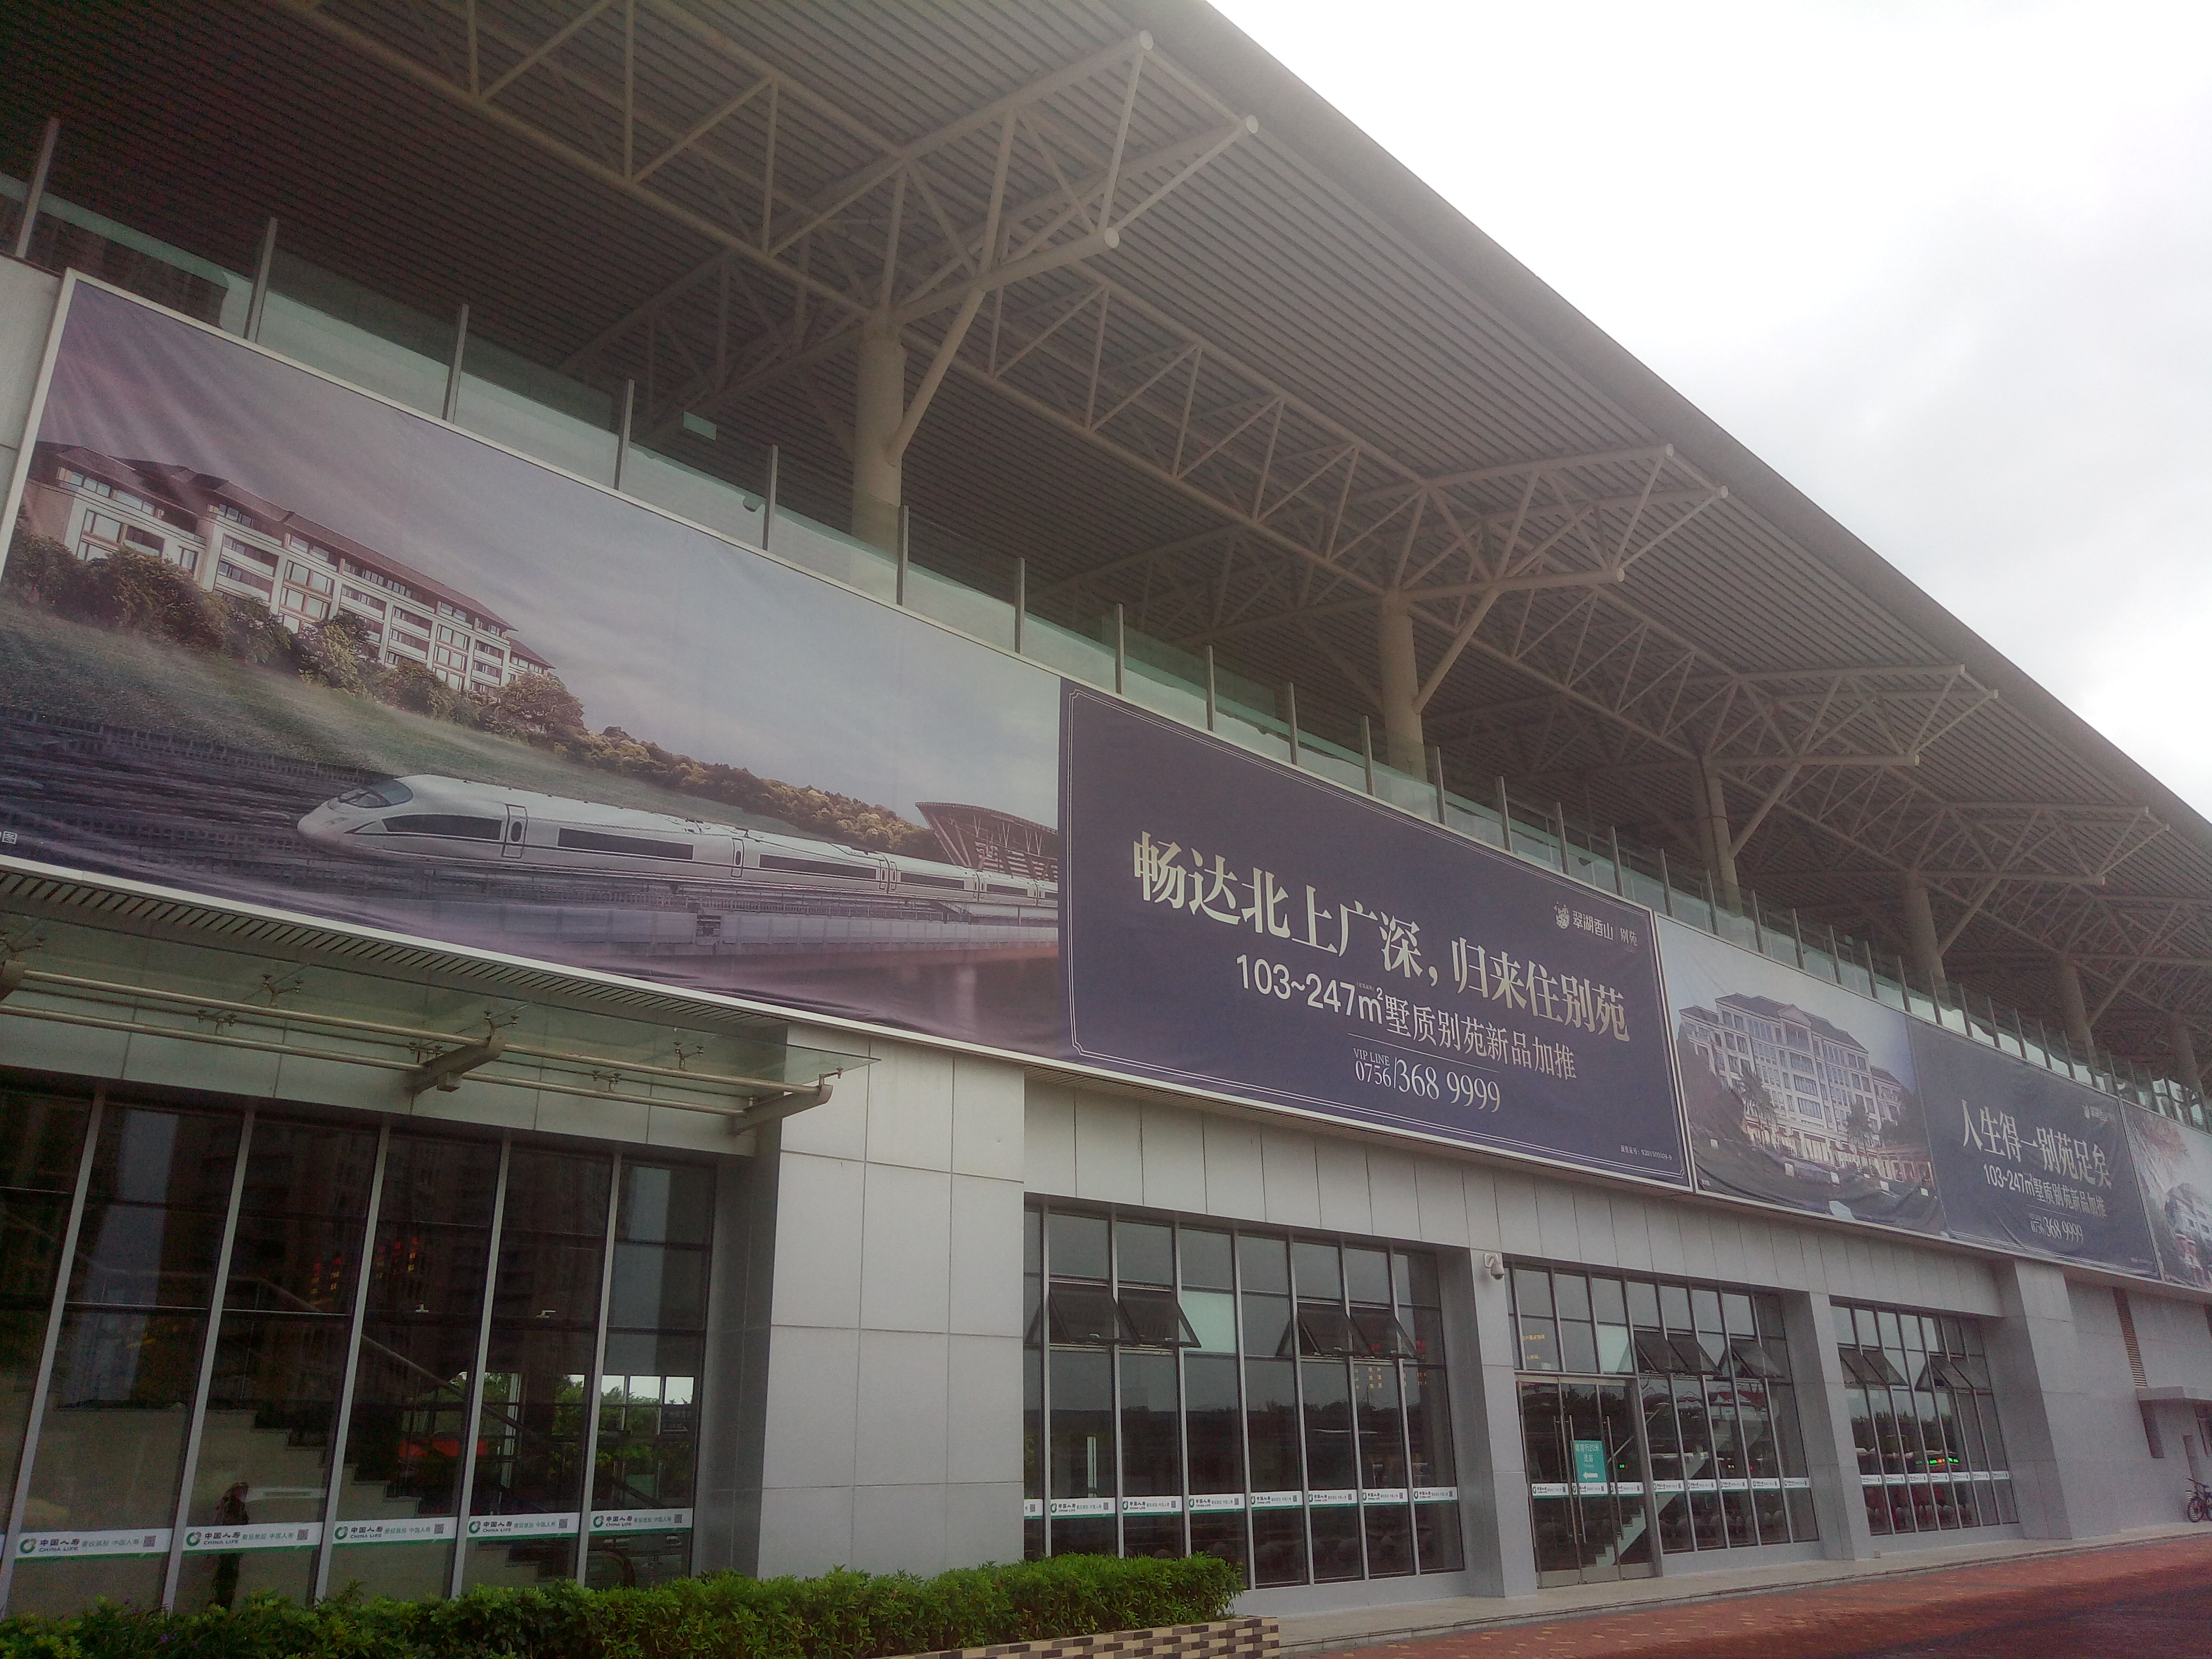
\includegraphics[width=0.48\linewidth]{Figures/Qualitative/tangjia}
	%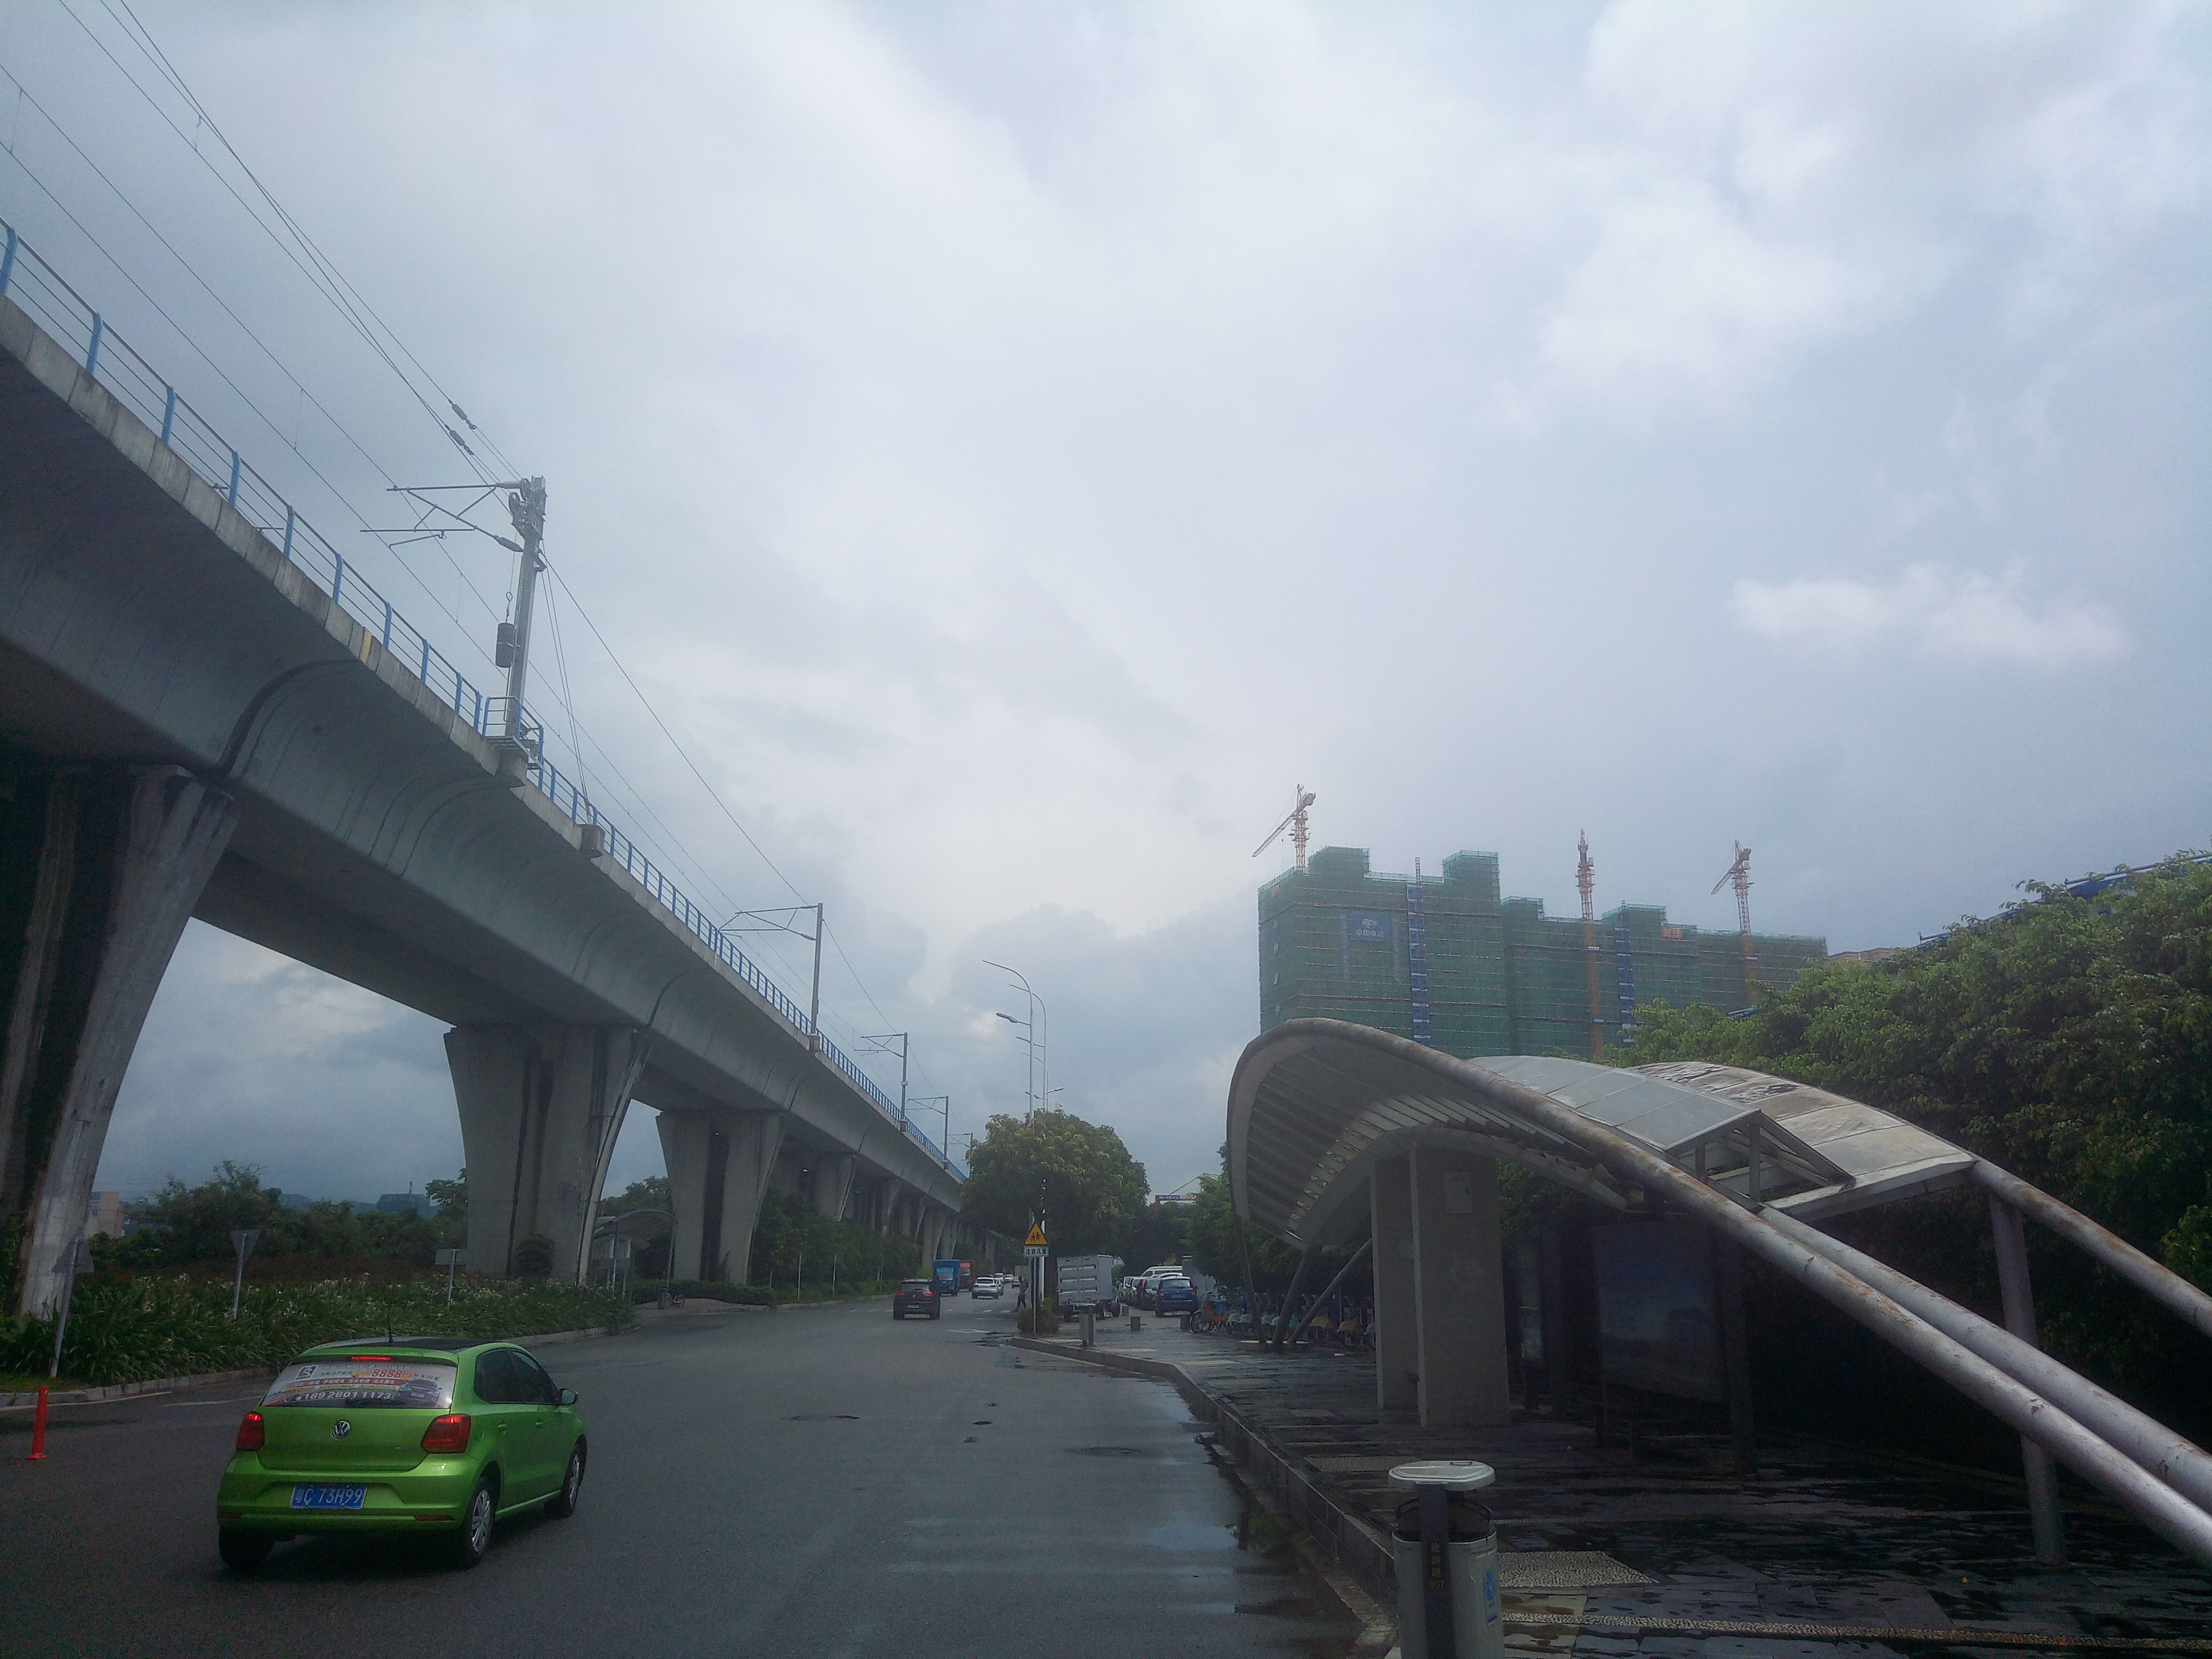
\includegraphics[width=0.48\linewidth]{Figures/Qualitative/zhuhai}\\
	%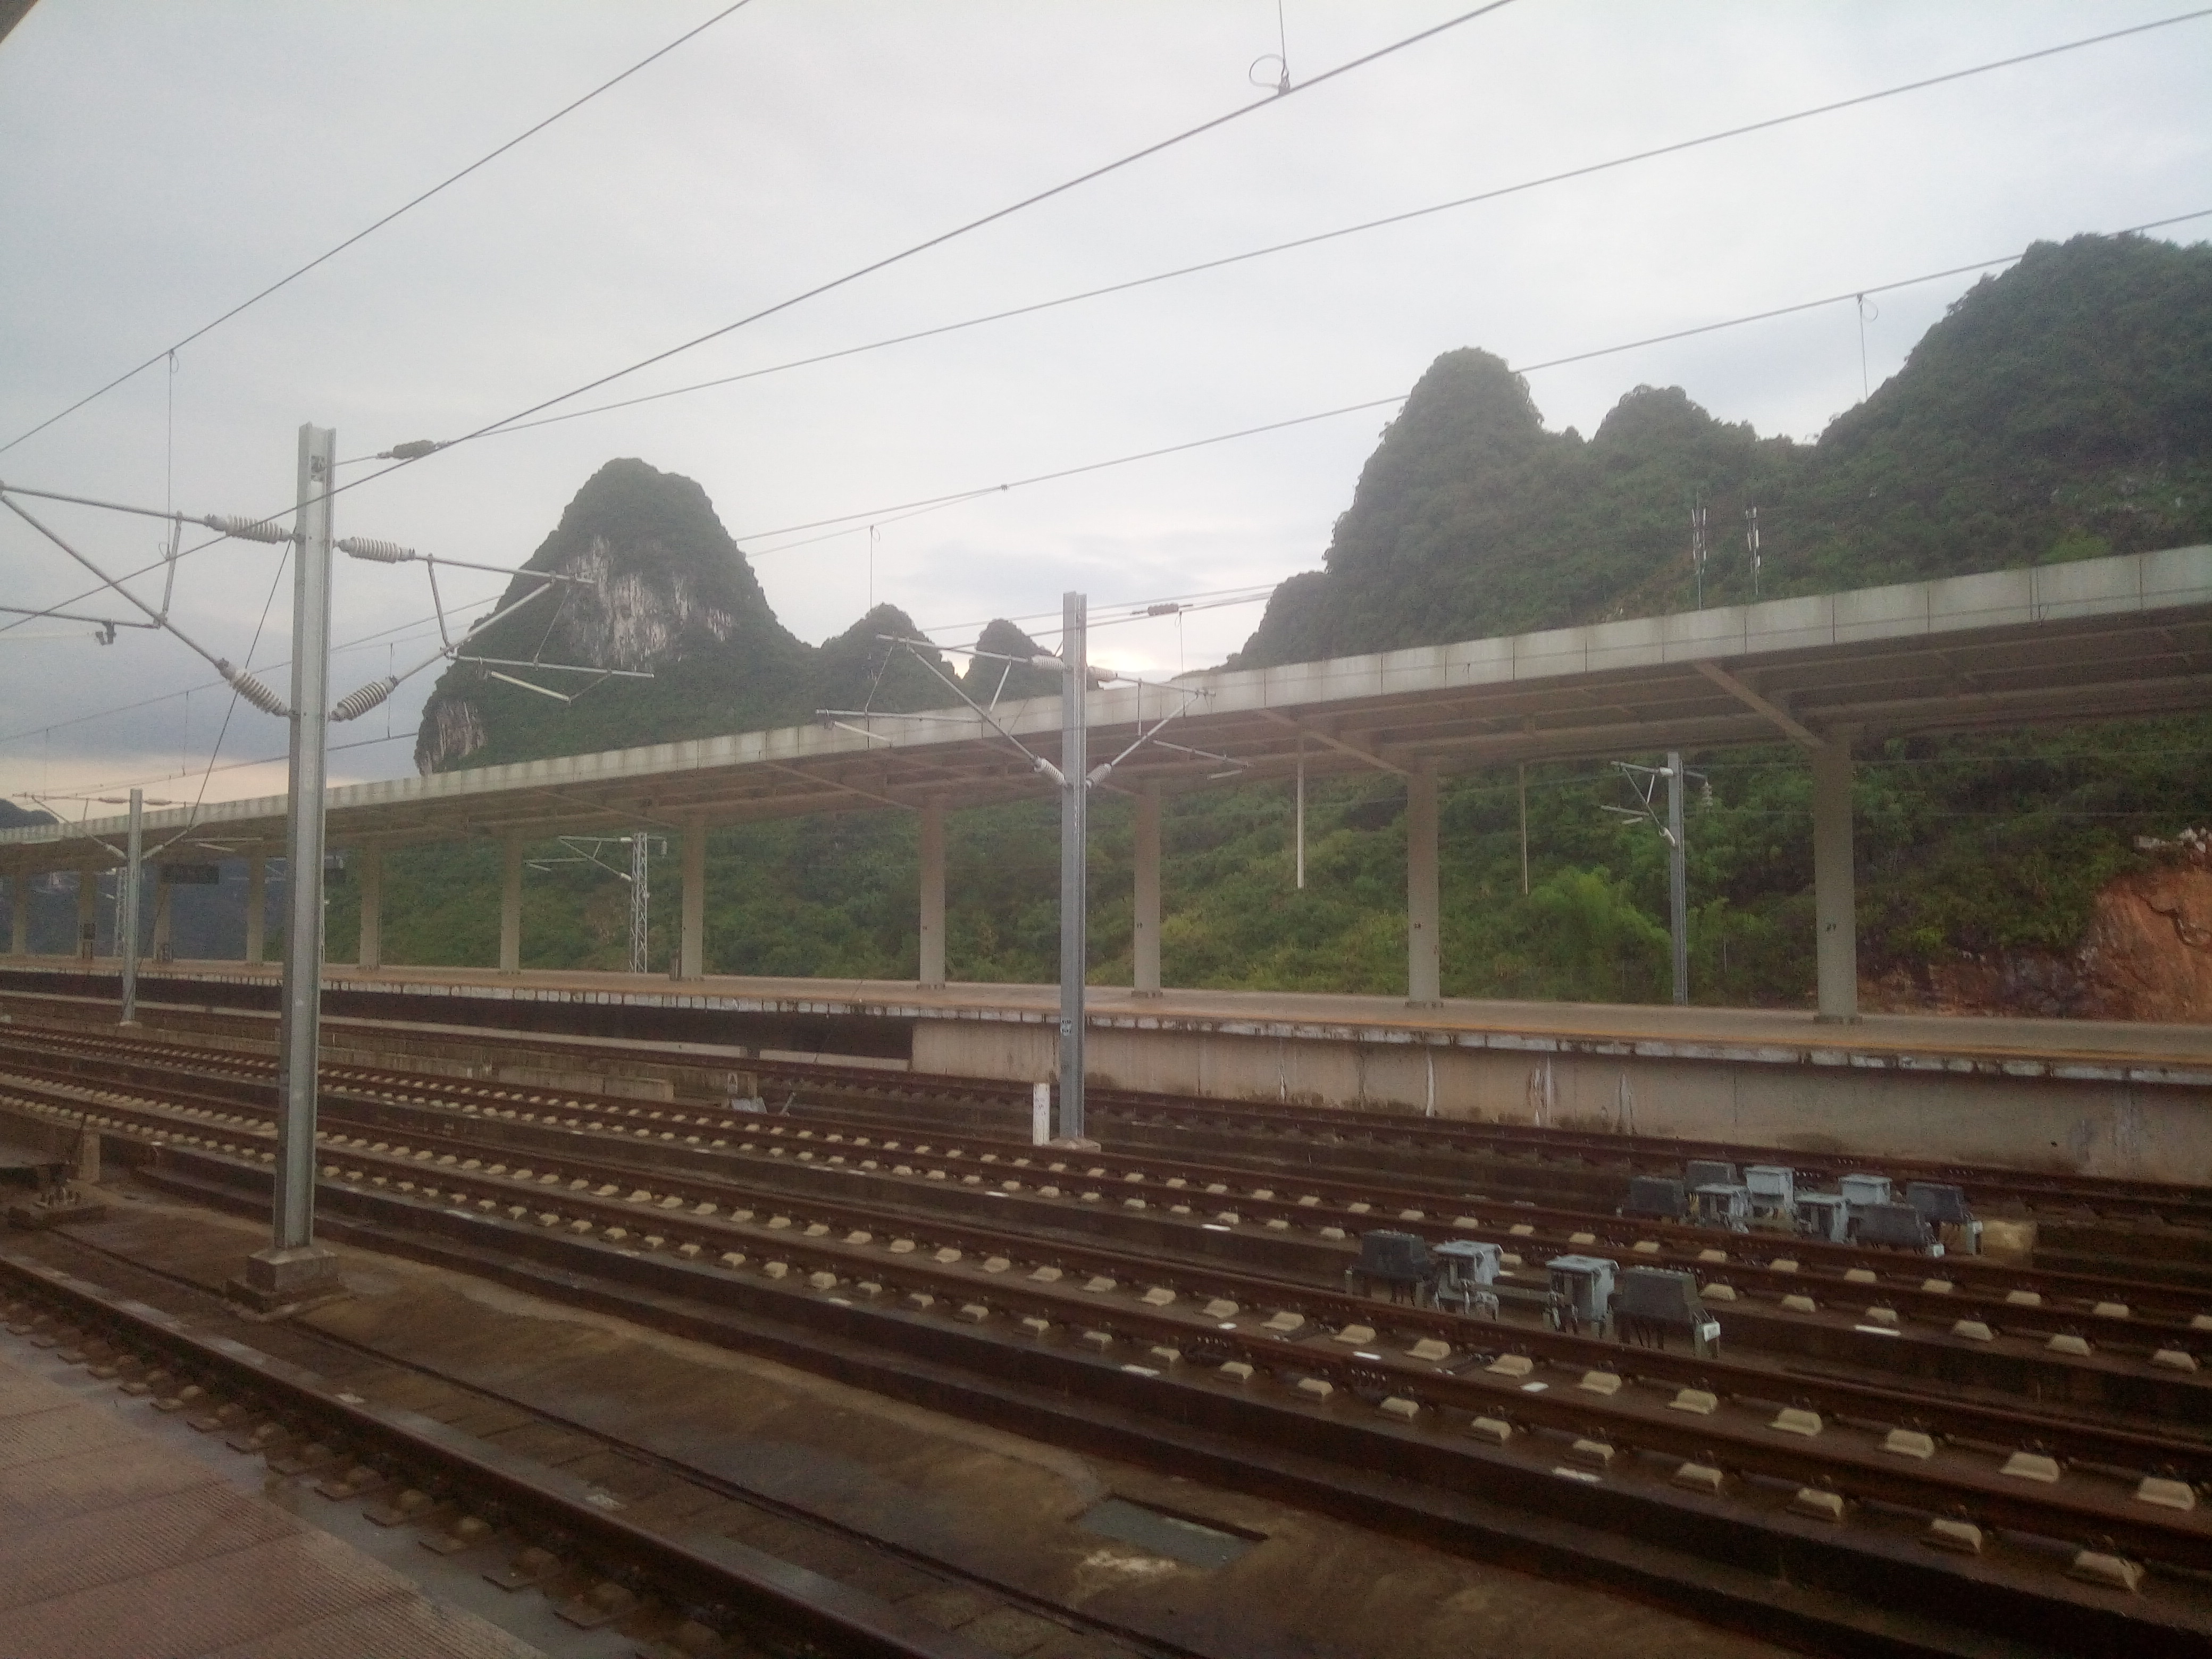
\includegraphics[width=0.48\linewidth]{Figures/Qualitative/yangshuo}
	%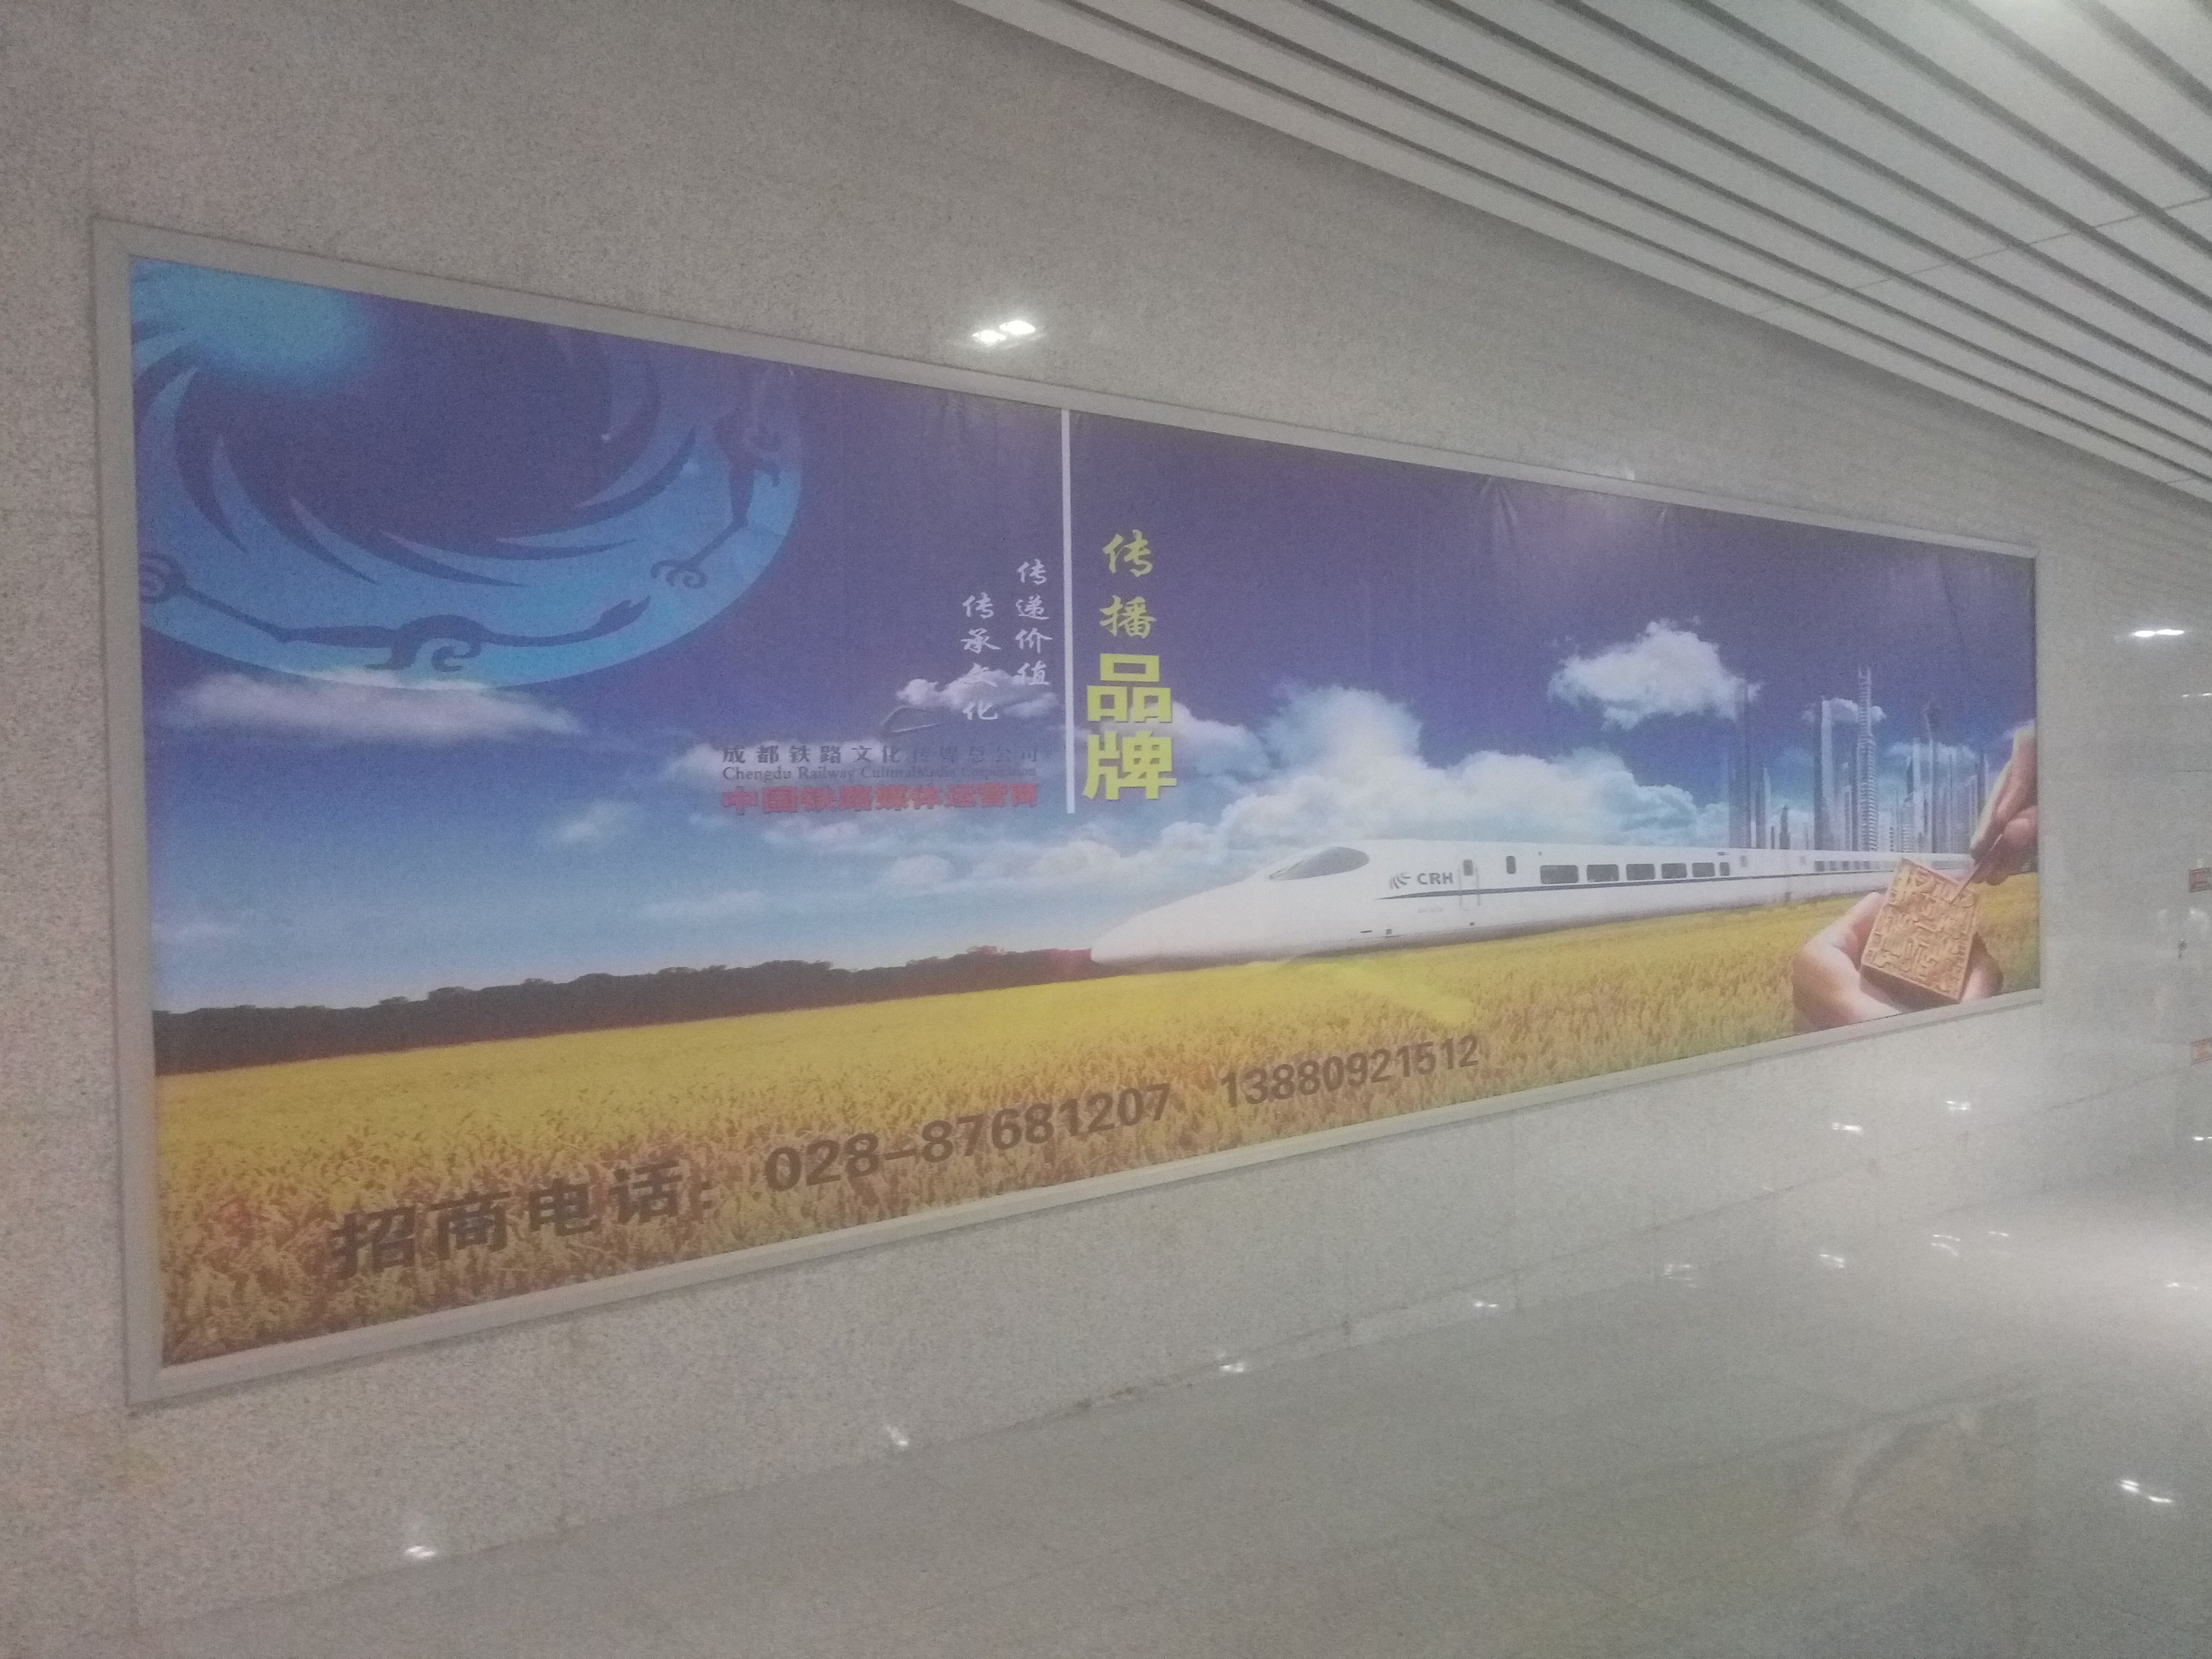
\includegraphics[width=0.48\linewidth]{Figures/Qualitative/chengdu}
	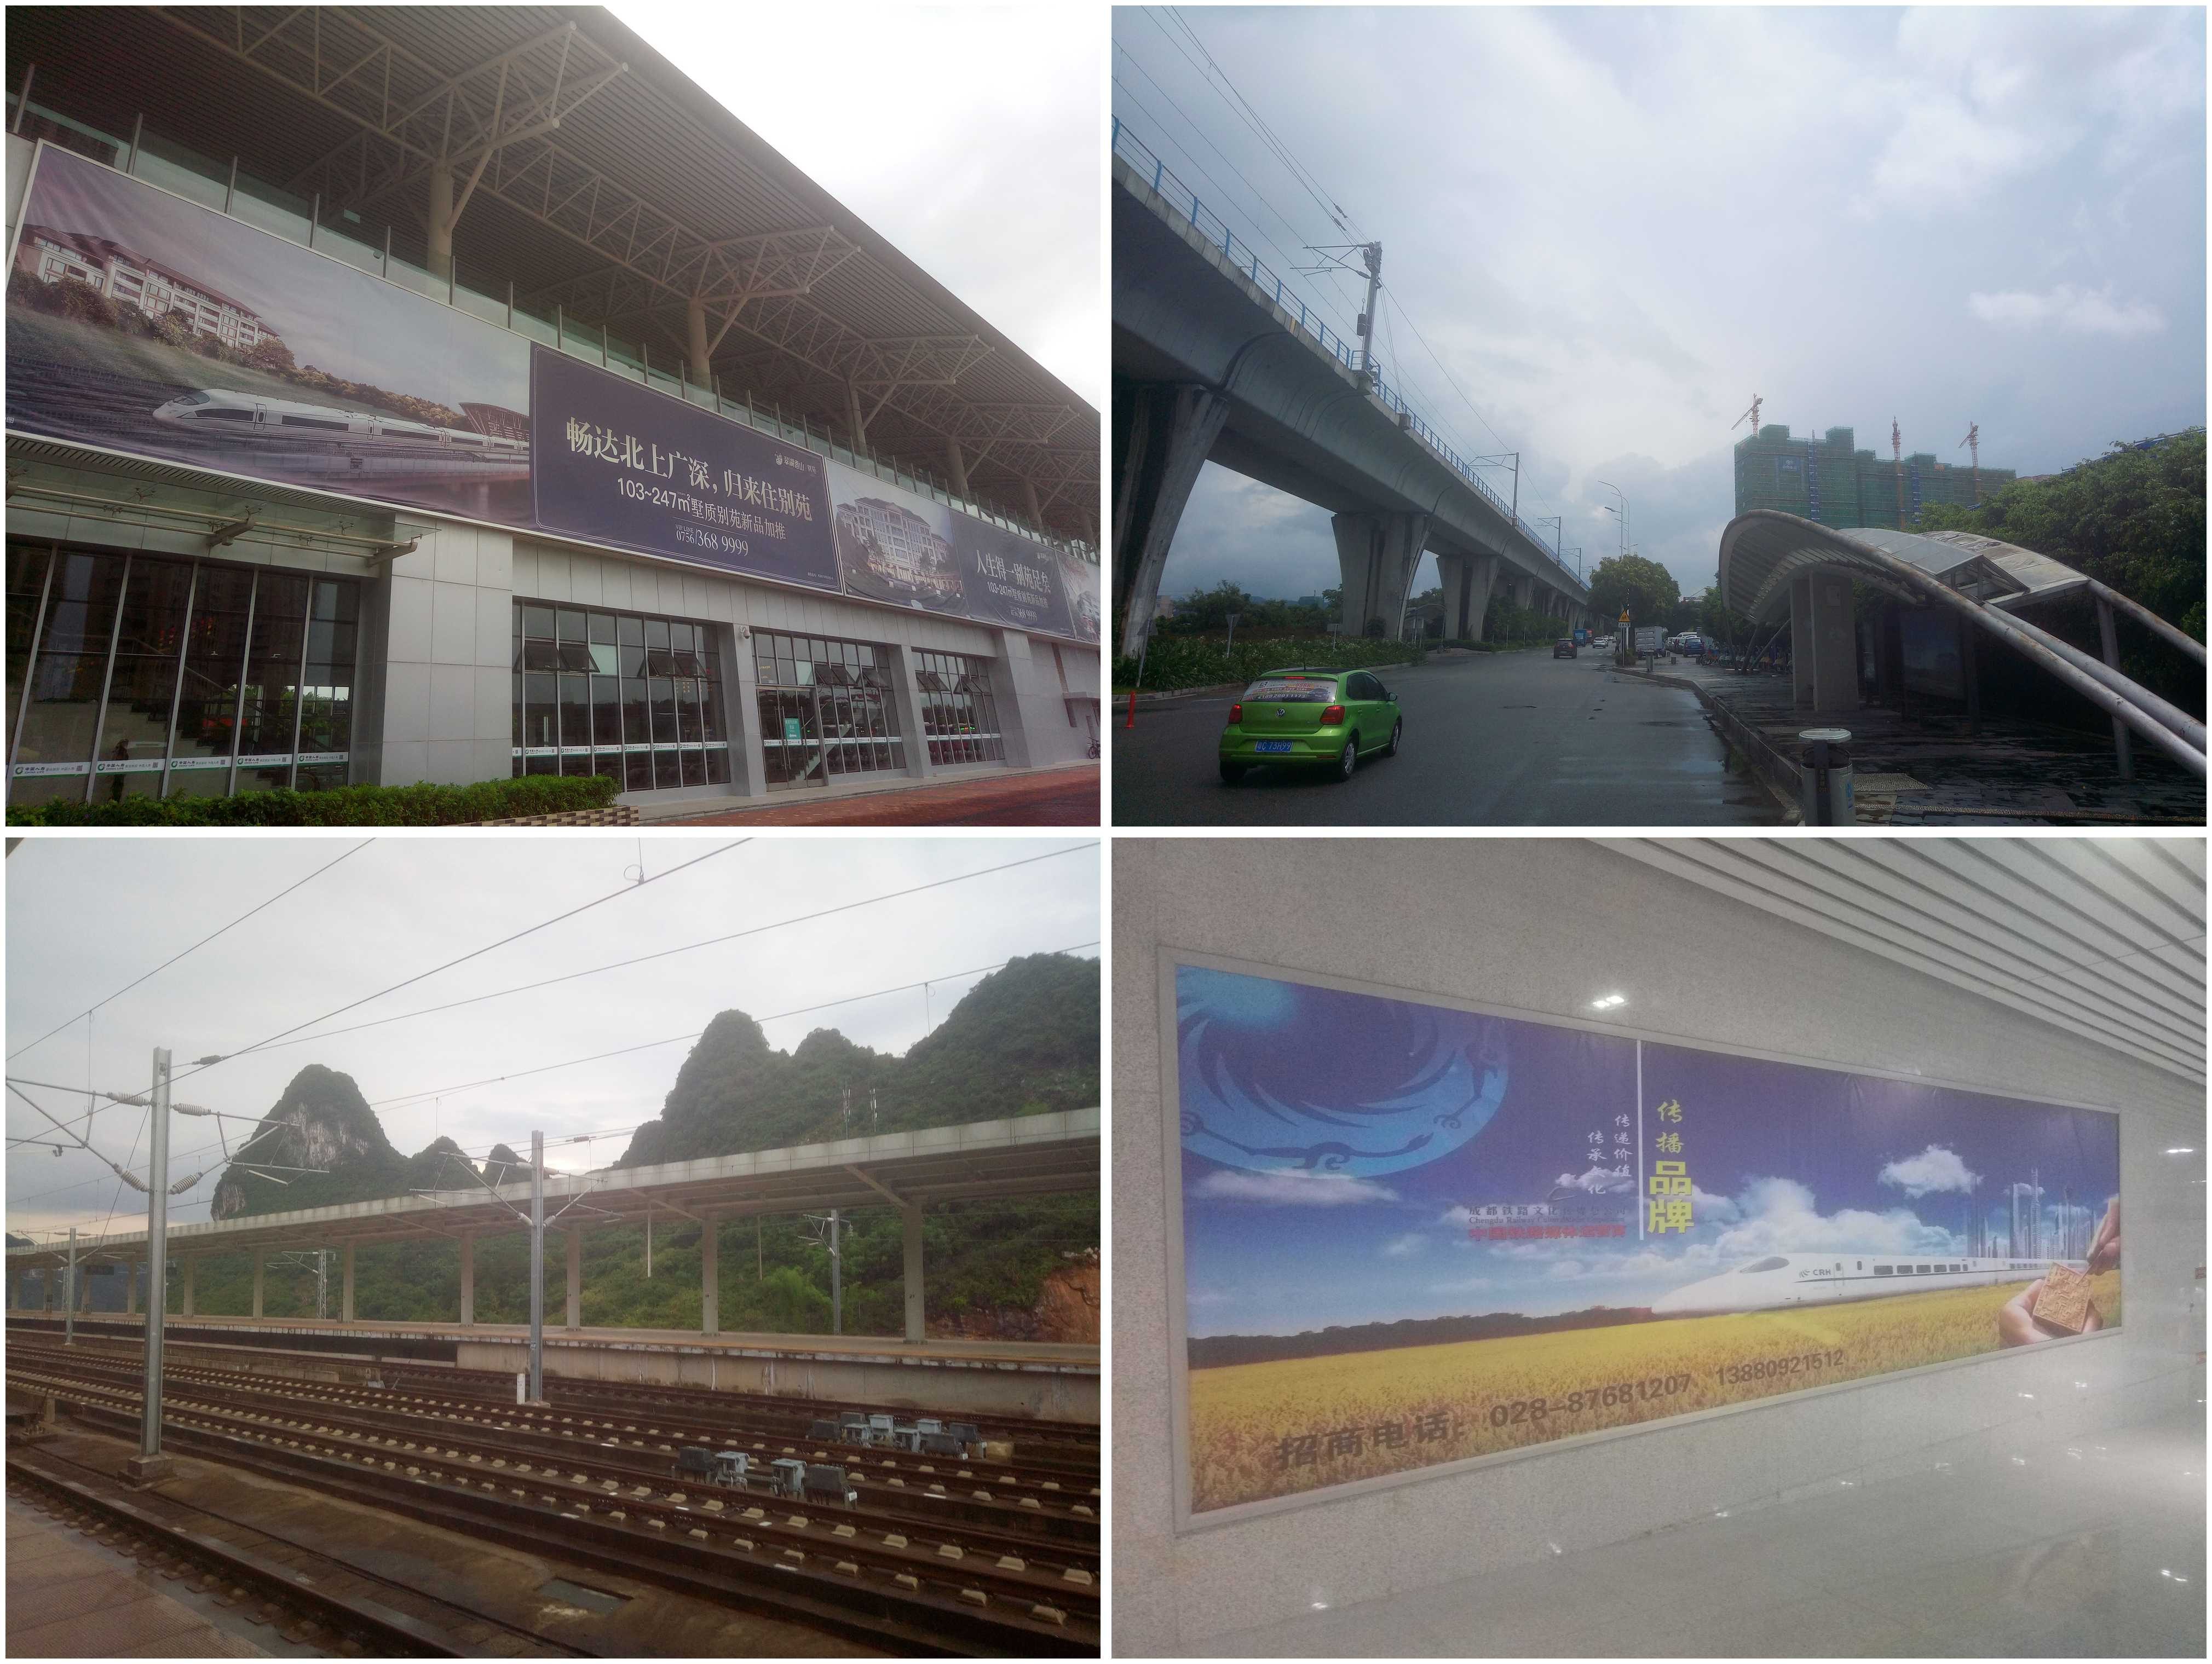
\includegraphics[width=\linewidth]{Figures/Final/1-3-1-fig-qualitative-hsr}
	\caption[][Réseau à grande vitesse en Chine]{(1)Tangjia HSR station in Zhuhai, with a huge advertisement for real estate suggesting the importance of the train connection, what can also be used as an argument for higher prices  (2) HSR line in Zhuhai, deserted bus station and new real estate project in a difficultly accessible area  (3) Yangshuo station, in the middle of nowhere on the High-speed line, recalling the “betterave-TGV” stations typical to France (4) Advertisement for HSR in Sichuan, at Chengdu international airport station on the line to Leshan and Emeishan. \label{fig:qualitative:hsr}}{\textbf{Manifestations locales des mutations induites par le nouveau réseau à grande vitesse.} \textit{(Haut Gauche)} Gare à grande vitesse de Tangjia, sur la commune de Zhuhai. La publicité monumentale pour une opération immobilière vante les mérites d'une proximité au réseau, qui est également utilisée comme un argument pour des prix plus élevés ; \textit{(Haut Droite)} Ligne à grande vitesse à Zhuhai, arrêt de bus déserté et projet immobilier en cours de réalisation dans une zone difficilement accessible\comment[FL]{difficile de comprendre le sens} ; \textit{(Bas Gauche)} La gare de Yangshuo, au milieu de nulle part \comment[FL]{trop rapide voir etudes sur les gares TGV en Espagne} sur la ligne à grande vitesse, rappelant les gares type ``betterave-TGV'' typiques en France ; \textit{(Bas Droite)} Publicité pour la grande vitesse dans le Sichuan\comment[FL]{quel rapport avec le developpement urbain ?}, à la gare de l'aéroport international de Chengdu sur la ligne vers Leshan et Emeishan.\label{fig:qualitative:hsr}}
\end{figure}
%%%%%%%%%%%%%






%%%%%%%%%%%%%%%%%%%%%
\subsection{Implementing TOD: contrasted illustrations}{Implémentation du TOD : des illustrations contrastées}


\bpar{
Regional branches such as the Guangzhou-Zhuhai line can be interpreted in-between a long distance service and regional proximity transportation, depending on the modulation of stop distribution. On top of that still exists the classical train network, and some connections require for now to use both and urban transportation, such as Zhuhai-Hong-Kong that I experimented by terrestrial transport only. The local urban network and real estate development operations are planned in close conjunction with the new train network : Zhuhai new tramway, of which a single line is today open and in test, aims at participating to a ``Transit-oriented development'' (TOD) approach of Urban Development which aims at promoting the use of public transport and a city with less cars, as claimed for example by the High-Tech Zone planning committee in charge of the development around Zhuhai North station. Observing the surroundings of Tangjia station, also constructed in the same spirit, the anti-urban atmosphere and unpractical setting can lead to question the effectiveness of the approach and wonder if it is not more a kind of self-fulfilling prophecy, as suggested by the advertisements for new real estate to sell highlighting the role of the train line. Other field observations, such as in Hong-Kong new territories, witness of an efficient and well achieved TOD, with the smart combination of heavy transit and local light rail, together with high urban densities around stations. These observations recall the complexity of urban trajectories coupled with network development, and how one must be careful before drawing any general conclusion from particular cases.
}{
Des branches régionales\comment[FL]{sens ?} du nouveau réseau à grande vitesse, comme la ligne Guangzhou-Zhuhai, peuvent être vues comme à l'intermédiaire entre un service a longue distance et un transport régional de proximité\comment[FL]{et alors ?}, en fonction de la modularité des motifs de desserte. A cela s'ajoute le réseau de train classique, et certaines connexions requièrent l'utilisation des deux réseaux et des transports urbains, comme la liaison entre Zhuhai et Hong-Kong expérimentée par voie terrestre seulement\footnote{à la suite du Typhoon Hato le 23/08/2017, les liaisons maritimes ont été interrompues pour une grande partie du delta.}. Le réseau urbain local et les opérations de développement immobilières sont planifiés en étroite conjonction avec le nouveau réseau de train : le tramway de Zhuhai, pour lequel une unique ligne est aujourd'hui ouverte et en phase de test, vise a participer à une approche par ``Transit-oriented Development'' (TOD)\comment[FL]{référence ?}[https://wenku.baidu.com/view/b1526461ff00bed5b8f31d01.html pour doc planning de xiaozhen] du développement urbain qui vise à favoriser l'utilisation des transports publics et une ville avec moins d'automobiles, comme voulu par exemple par le Comité de Planification de la \emph{High-Tech Zone} en charge du développement autour de la gare nord de Zhuhai. L'observation des alentours de la gare de Tangjia, également construite dans le même esprit, une certaine atmosphere anti-urbaine\comment[FL]{sens ?} et une organisation peu pratique peut mener au questionnement de l'efficacité de l'approche et a des interrogations sur la nature auto-prophétique du projet, comme suggéré par les publicités pour du nouvel immobilier a vendre, \comment[AB]{pas très comprehensible} appuyant sur l'importance de la presence de la ligne ferroviaire. Toute une narration autour du TOD, parfois sans réel fondement empirique\comment[FL]{qu'est ce qu'il pourrait y avoir comme fondement empirique ?} dans le cas donné, semble être utilisée par différents acteurs du développement. D'autres observations de terrain, comme dans les \emph{new territories}\comment[FL]{trad.} a Hong-Kong, témoignent d'un TOD efficace et réalisant son objectif, avec une combinaison intelligente\comment[FL]{sens ?} entre transport lourd et tramway local léger, ainsi qu'une grande densité urbaine autour des gares. Ces observations rappellent la complexité des trajectoires urbaines couplées au développement du réseau, et qu'il s'agit d'être prudent avant de tirer toute conclusion générale a partir de cas particuliers. Nous résumons en Fig.~\ref{fig:qualitative:schema} la comparaison des deux cas de TOD évoqués ci-dessus, sous forme de schéma synthétique des grandes lignes urbanistiques de chacune des zones. A Hong-Kong, les zones urbaines ont été planifiées conjointement\comment[FL]{cette discussion est pertinente mais il faut justifier (?)} avec la ligne du MTR (transport lourd) et les multiples lignes de tramway léger, dont l'infrastructure et l'organisation des missions permettent de rejoindre rapidement la gare la plus proche, distribuant une accessibilité très uniforme pour l'ensemble des quartiers du territoire. Au contraire à Zhuhai, le village de Tangjia est ancien, antérieur même à l'ensemble du reste de Zhuhai, qui s'est développé sans articulation particulière avec les infrastructures de transport. Le tracé du tramway, qui vient d'ouvrir, prend avantage du tracé de la nouvelle ligne ferroviaire, pour essayer de reorganiser le nord de Zhuhai\comment[FL]{un peu simpliste}, et en particulier la High-tech Zone qui s'étend de la gare du Nord (Zhuhai Bei) à Tangjia. Actuellement, l'organisation urbaine porte toujours les stigmates \comment[FL]{sens ? (concretement ?)} de cette mise en place déphasée, et l'accessibilité en transport en commun est relativement faible, les lignes de bus étant sujettes à une congestion croissante due à la forte augmentation du nombre d'automobiles. Cet exemple de terrain nous démontre ainsi que (i) sous la même qualification existent des processus très différents, extrêmement dependants aux particularités géographiques, politiques, économiques ; et que (ii) la mise en place d'un territoire fonctionnel en termes d'accessibilité nécessite une articulation fine qui semble résulter d'une approche de planification intégrée réalisée sur le temps long.
}



%%%%%%%%%%%%%
\begin{figure}
	\includegraphics[width=\linewidth]{Figures/Qualitative/tod}
	\caption[TOD in Hong-Kong and Zhuhai][TOD à Hong-Kong et Zhuhai]{\textbf{Comparative analysis of two implementations of TOD in PRD.}\label{fig:qualitative:schema}}{\textbf{Analyse comparative de deux implémentations du TOD \comment[FL]{si ca jour un role important dans ton discours, tu dois le definir}[(JR) fait en 1.1] en PRD.} A une échelle comparable, nous synthétisons la configuration urbaine de Yuenlong (\cn{元朗}) et Tuenmun (\cn{屯门}), Hong-Kong New Territories (\cn{香港,新界}), et de Xinwan, Xiangzhou, Zhuhai (\cn{珠海,香洲,新湾}), qui contient la High-Tech zone de Zhuhai dans sa partie nord en particulier. Les configurations témoignent de dynamiques d'articulation différentes, et des temporalités de construction décalées, révélant ainsi diverses réalités sous la notion de TOD. Une première interprétation serait que celle-ci est efficace si la trajectoire du système territorial complet (aménagement urbain et réseau de transport) est infléchie tôt dans sa genèse, tandis qu'un système avec un certain niveau de maturité sera plus inerte.\label{fig:qualitative:schema}\comment[FL]{traduire la carte ; traduire ; }\comment[AB]{$\rightarrow$ realisation : x ?}}
\end{figure}
%%%%%%%%%%%%%




%-------------------------

%%%%%%%%%%%%%%%
%\subsection[Floating Observation][Observation Flottante]{An Experiment in Floating Observation}{Une Experience en Observation Flottante}
\subsection{Floating Observation}{Observation Flottante}


\bpar{The devil is in the details, and transportation systems are a typical embodiment of this image. What some will see as detail contains the majority of information for others. Logically trapped in a scientific information bubble, despite all the positions developed in introduction, we must stay aware of the nature and the range of knowledge produced here. What can be called detail in our case, for an accessibility study of a transportation network for example, such as subjective views of users or social relations inducted by the situations consequent to the dynamics of the transportation system, will be at the center of the questioning for some viewpoints in anthropology or sociology. Such knowledge, that could surely find a way in our work, is out of scope because of the lack of long-time fieldwork. We propose here however to sketch such a qualitative entry, to suggest directions for future research and better understand processes in a concrete way.}{
%Si le diable est dans les détails, les systèmes de transport entre autres sont l'allégorie de cette adage. Ce que certains appellent détail contient la majorité de l'information pour d'autres. Logiquement enfermés dans une bulle scientifique, malgré toutes les volontés développées en introduction, on tâchera de rester conscient de la nature et la portée de la connaissance produite ici. Ce que nous pourrions appeler détail, lors de l'étude de l'accessibilité d'un réseau de transport par exemple, tel des impressions ressenties par les usagers ou les relations sociales induites par les situations découlant des dynamiques du systèmes, seront le centre du questionnement pour un anthropologue ou sociologue. Une telle connaissance, qui trouverait certainement une place dans nos problématiques, est hors de notre portée de par l'absence de terrain de longue durée. \comment[FL]{c'est TB ce que tu ecris \ldots mais a supprimer de la these}
Nous proposons à présent d'ébaucher une entrée qualitative d'un certain type, pour suggérer une façon de compléter nos connaissances et mieux cerner les processus de manière concrète.
}


\bpar{}{
L'entrée prise suit la méthode \emph{d'observation flottante}, introduite à l'interface de l'anthropologie et la sociologie par~\cite{petonnet1982observation}, avec l'ambition de fonder une anthropologie urbaine, au sens de l'étude des comportements humains au sein d'un environnement urbain. Il ne s'agit pas exactement de la même idée que l'anthropologie de l'espace de \emph{Choay}~\cite{choay2009pour} qui explore la direction inverse, c'est à dire le propre des sociétés humaines de façonner l'espace, et la capacité de construire un environnement bâti à différentes échelles par l'architecture et l'urbanisme. Notre contexte méthodologique est le suivant Répondant à un besoin de mouvement que le sédentaire éprouve facilement, le chercheur se place au centre du processus de production de connaissances, nous citons, en ``rest[ant] en toute circonstance vacant et disponible, à ne pas mobiliser l'attention sur un objet précis, mais à la laisser flotter afin que les informations la pénètrent sans filtre, sans a priori, jusqu'à ce que des points de repère, des convergences, apparaissent et que l'on parvienne alors à découvrir des règles sous-jacentes''. Cette méthode peut servir d'étude préliminaire pour fixer des protocoles et grilles précises d'entretien : elle est par exemple utilisée justement au sujet du transport par~\cite{de2012deplacements}. Nous nous en servons dans notre cas comme méthode d'extraction de faits stylisés, afin d'informer des exemples de processus d'interactions directement visibles.
}



\paragraph{Methodology}{Méthode}

\bpar{}{
Les mouvements pendulaires à échelle moyenne\comment[FL]{c'est quoi ?} sont nécessairement vécus d'une façon particulière en comparaison à d'autres lieux géographiques et à d'autres échelles sur le même lieu. Et si une façon d'appréhender des faits stylisés particuliers était alors d'effectuer l'analogue d'une étude de perturbation sur le système, mais en prenant comme référentiel l'observateur lui-même ? Il s'agirait de faire porter un choc sur une situation ``d'équilibre'', puis de se laisser flotter au gré du courant pour appréhender la réaction et certains mécanismes qu'il aurait été difficile de considérer en suivant sa routine. Une expérience naturelle causée par une perturbation des transports (qui en région francilienne est bien courante\comment[AB]{et pas en Chine ? :)}) est un événement provoquant une expérience naturelle, au sens où le chercheur peut capturer des situations et réactions individuelles particulières.\comment[FL]{il y a sans doute une amorce de travail interessant \ldots plutot en dernier chapitre, exploratoire du type ``pour aller au dela''} Notre méthodologie est relativement simple : déambuler dans les transports en commun, avec ou sans but et de manière ou non aléatoire, mais en essayant sur chaque trajet de maximiser les opportunités de mise en situation ou de capture d'évènement, typiquement en évitant un trajet de routine\footnote{Cette contrainte sera respectée dans notre cas pour le Guangdong, mais pas pour l'Ile-de-France.}. La répétition de l'expérience visera également à maximiser la couverture spatiale, temporelle, de situation. Une production traçable est en théorie nécessaire à chaque itération, qu'il s'agisse de description factuelle, de description perçue, de semi-synthèse. Celle-ci permet a posteriori de voir les stratifications successives du vécu et des expériences d'observation progressivement raffinées dans leur contexte, et de tracer ainsi la genèse des idées induites. Nous faisons le choix de retranscrire l'aspect subjectif, voir maximiser celui-ci dans les synthèses générales des observations, afin d'appuyer cet aspect en contraste avec la suite de notre travail qui sera relativement déconnecté du sujet menant la recherche, et en echo avec les recommandations de \cite{ball1990self} pour la place de la subjectivité dans la recherche ethnographique de terrain.
}




%%%%%%%%%%%%%%%%%%%
\begin{figure}[h!]
\begin{mdframed}
Le ciel est gris et les visages fermés, Oxmo \comment[AB]{est-ce une figure de style? je ne comprends pas bien le principe sinon: c'est bien toi qui flotte non ?} avait tristement raison, ce Soleil du Nord n'avait de lumière que le nom. L'initié ne saura s'y tromper et ressentira au fond de lui-même cette banale routine d'un aller-retour quotidien en RER. Il ne cherchera ni à maudire les planifications successives dont les stratifications temporelles ont laissé décanter cette organisation territoriale incongrue, ni à se prendre à rêver d'une trajectoire de vie alternative puisque choisir c'est un peu mourir et qu'il ne se sent pas une âme de Phoenix aujourd'hui. Peut être que la beauté de la ville est finalement dans ces tensions qui la façonnent à tous les niveaux et dans tous les domaines, ces paradoxes qui deviennent cadre de vie au point d'asséner quotidiennement une vérité. Cette philosophie de couloir de métro, le francilien en fait son cheval de bataille car après tout s'il vit en ville il doit bien la connaître. Encore un rail cassé sur le A, ``tout cela est mal géré, et ce réseau est mal conçu'' vocifère un utilisateur journalier, s'improvisant expert en planification ; d'autres plus patients prennent leur mal en patience mais se présentent tout aussi connaisseurs d'une illusoire vision d'ensemble d'un territoire aux multiples visages. Ces usagers \emph{sont} pourtant le système, de manière concrète à leur échelle d'espace et de temps, par induction et émergence aux échelles supérieures. La fourmi est supposée ne pas avoir conscience de l'intelligence collective dont elle est une des composantes fondamentales. Ils n'ont de la même manière que peu de perception de l'auto-désorganisation dont ils sont la source, peut-être la cause, et qui très sûrement subissent les désagréments de ses dynamiques. Se laisser flotter dans les transports franciliens est une expérience intemporelle. Presque thérapeutique parfois, quand l'un commence à perdre son optimisme quant à l'intérêt d'une vie urbaine, une excursion aléatoire en métro rappelle rapidement la richesse et la diversité qui sont un des plus grand succès des villes. C'est cette variété apparente de profils que le chercheur retiendra principalement de ces errements dont la méthodologie est de ne pas avoir de méthodologie\comment[FL]{non : il y a quelque chose derriere}, et il gardera à l'esprit qu'il n'existe pas d'échelle où un traitement spécifique de chaque objet géographique n'est pas nécessaire : en quelque stations sur la ligne 4 le profil des quartiers et donc des usagers\comment[FL]{attention a ce racourci glissant (tres)} change profondément et souvent sans transition au moins trois fois, comme sur la ligne 13 nord où les motifs horaires soulignent d'autant plus de dures réalités socio-économiques qui sont en fait géographiques dans cet \emph{espace produit} de la métropole. Lorsqu'il s'agit de modéliser, prendre en compte les limites de toute tentative de généralisation est d'autant plus cruciale comme chaque modèle est un équilibre fragile entre spécificité et généralité.\comment[FL]{c'est interessant : a enrichir}

\medskip

\noun{Encadré : } \textit{Une expérience en observation flottante en région parisienne}
\end{mdframed}
\end{figure}
%%%%%%%%%%%%%%%%%%%




%%%%%%%%%%%%%%%%%%%
\begin{figure}[h!]
\begin{mdframed}
Le trajet sera long. La perturbation choisie est la simulation de l'événement malencontreux, ``\cn{我的护照丢了,我得去法国的领事馆在广州}'' \comment[FL]{tu n'es pas aidant avec le lecteur}: la perte de son passeport en Chine est assurément malencontreuse, puisque l'intégralité des trajets interurbains y est conditionnée. Traverser la mega-région urbaine du sud vers le nord pour rejoindre Guangzhou dans cette situation relève du défi. De bus urbain en bus urbain, des terminus plus ou moins bien articulés. Un village traditionnel factice est sorti de terre pour faire le bonheur des touristes, non loin de la maison natale de Zhongshan, peu crédible vu l'accessibilité. Des contrastes saisissants et un paysage très hétérogène, des enclaves de pauvreté dans des zones nouvellement prisées. Les relocalisations plus ou moins volontaires vers les franges façonnent un nouveau paysage d'inégalité géographique que l'on connait déjà bien en Europe. A l'image de cet embouteillage continu, la réinvention de la ville déjà bien avancée ici se doit de faire des choix cruciaux pour être l'exemple d'une trajectoire durable. Une résilience impressionnante des usagers à une perturbation majeure, une capacité d'auto-organisation locale rendant fonctionnels des aménagements qui auraient pu ne pas l'être : de Shenzhen, Baoan à Zhuhai, Tangjia ou à Zhongshan, Xiaolan, la flotte de moto-taxis informels sauve l'accessibilité locale, comme me le confirme Jingzi habitant le sud de Zhongshan et étudiant au nord de Zhuhai et pour qui le train est une solution de mobilité même pas envisagée. Du tramway au BRT, choix et compromis équivalents ? Le premier étonne plus les nouveaux usagers. Peut être aussi un argument percutant pour valoriser le complexe spécialement conçu autour du terminus. Les choix locaux sont d'autant plus différentiables qu'il est difficile de passer d'une zone à l'autre. Bloqué non loin de Guangzhou, le pont est fermé, le métro est en face mais impossible de le rejoindre. Juste le temps pour se rabattre sur la gare de Xiaolan et retour à la case départ, défi bien loin d'être réalisé. Observer l'adaptabilité ne suffit pas à la développer ? Des pratiques de mobilité très vite adaptées par les usagers : des trains à grande vitesse bondés en toute heure de la semaine, semble-t-il pour des motifs très divers. Un développement territorial apparent, des impacts à moyen terme qu'on peut parier non discutables. Si la structure est intégrée et flexible, discuter d'effets structurants devient une tautologie puisque la trajectoire du système urbain devient alors l'aspect plus ou moins contrôlable, selon les échelles de temps et d'espace.


\medskip

\noun{Encadré : } \textit{Une expérience en observation flottante, Guangdong, Zhuhai}
\end{mdframed}
\end{figure}
%%%%%%%%%%%%%%%%%%%



\paragraph{Results}{Résultats}

Nos séquences d'observation de terrain ont eu lieu d'une part en Chine, majoritairement dans le Guangdong à Zhuhai, lors de sessions dédiées. Les observations s'étendent entre le 10/10/2016 et le 23/01/2017 ainsi qu'entre le 08/06/2017 et le 01/09/2017. Le mode de transport majoritaire est le bus de ville, suivi par le train régional, puis le train à grande vitesse et le ferry ; la portée des déplacements correspondent à celle des modes. Les compte-rendus détaillés, écrits à la volée de manière subjective et édités a posteriori le moins possible, comme expliqué précédemment, sont disponibles en Appendice~\ref{app:sec:qualitative}. Les observations pour la région parisienne sont quasi-quotidiennes et non consignées ; celles-ci ont eu lieu en plus grande partie sur la ligne 4 du métro et sur la ligne A du RER entre février 2016 et octobre 2016, sur la ligne R du Transilien et la ligne A du RER entre novembre 2016 et septembre 2017 puis entre février 2017 et mai 2017, puis sur la ligne 9 et la ligne 4 entre septembre 2017 et octobre 2017.

\comment[FL]{ce qui me frappe ici c'est que tu ne parles que de transport et pas de ville ; donc pas de coevolution. pourtant il y a certainement des marqueurs de coevolution a observer de visu (ex gare neuve avec immeubles neufs). D'autre part tu dis ne pas avoir de methode. c'est mal dit, ok pour la demarche ``souple''. par contre tu dois avoir une question, ou au moins des reponses. la tu n'offres pas de cadre de lecture de tes propos.}

Les deux synthèses d'observation flottante pour chacune des régions, matériaux produit à partir des notes brutes, sont présentées dans les encadrés ci-dessus. Celles-ci illustrent entre autre par des exemples subjectifs certaines instances d'interactions entre réseaux et territoires, majoritairement aux échelles microscopique et mesoscopique, pour des processus touchant à la mobilité. La subjectivité et l'interprétation permet aussi d'extrapoler sur des processus à plus grande échelle, en terme d'accessibilité par exemple. Ceux-ci ne peuvent toutefois être pris plus que comme une illustration et introduction thématique. Par une prise de recul, nous proposons de lister certains enseignements qui peuvent être tirés de cette expérience à un niveau méta :

\begin{enumerate}
	\item La complexité du système de transport et de son intégration dans le système territorial\comment[FL]{tu donnes un angle non symmetrique} peut avoir des conséquences divergentes en termes de performance finale, et par exemple de soutenabilité. Dans le cas Chinois, l'auto-organisation et l'adaptabilité locale sont des atouts de l'efficacité émergente\comment[FL]{defs}, tandis qu'en France la complexité semble être source de freins et finalement d'externalités négatives. \comment[FL]{tres schematique, enrichir}\comment[AB]{différence vient-elle en partie de l'adaptabilité différentielles des populations ? (ie origine culturelle)}
	\item La résilience, qui peut être caractérisée par exemple \comment[FL]{pas d'accord avec ta definition} par la vitesse de mutation des pratiques de mobilité et reliée à l'adaptabilité, semble également très sensible aux particularités géographiques.
	\item La question des échelles de temps et d'espace observables, ce qui conditionnera partiellement celles qu'on peut modéliser, est ambiguë dans l'observation, comme le témoigne l'observation conjointe de la mobilité et de manifestation de motifs d'accessibilité.
	\item La comparabilité des cas et des situations géographiques est, dans notre cas, mais a priori plus généralement, un point épineux auquel il n'existe pas de solution idéale. Le compromis entre généralité et particularité est alors déterminant dans la construction d'une théorie et de modèles géographiques. \comment[FL]{pourquoi soulever cette question ? tu ne fais pas de comparaison dans ta these. par contre une vraie question est la tranposabilite des approches de modelisation d'un territoire a un autre.}
\end{enumerate}


Ces considérations participeront à l'orientation des postures ontologiques et épistémologiques que nous prendrons par la suite.

\comment[FL]{manque litérature ``de base'' sur interactions ville/transport.}

\comment[FL]{transport - territoire : majorite sur transport ?}


\stars




